\documentclass[11pt,letterpaper]{article}
\usepackage[margin=0.85in]{geometry}
\usepackage[T1]{fontenc}
\usepackage{lmodern,microtype,amsmath,amssymb,booktabs,graphicx}
\usepackage[font=small,labelfont=bf]{caption}
\usepackage{titlesec,fancyhdr}
\usepackage[colorlinks=true,linkcolor=blue!50!black,urlcolor=blue!50!black,citecolor=blue!50!black]{hyperref}
\usepackage{xcolor}
\hypersetup{pdftitle={ODE-FFN: Progress Report 1}}
\setlength{\parindent}{0pt}
\setlength{\parskip}{5pt}
\renewcommand{\topfraction}{0.98}
\renewcommand{\textfraction}{0.01}
\renewcommand{\floatpagefraction}{0.8}
\titlespacing*{\section}{0pt}{9pt}{4pt}
\titleformat{\section}{\large\bfseries}{\thesection}{.6em}{}
\pagestyle{fancy}
\fancyhf{}
\fancyhead[L]{\small ODE-FFN: Progress Report 1}
\fancyhead[R]{\small 20 October 2026}
\fancyfoot[C]{\thepage}
\setlength{\headheight}{14pt}
\newcommand{\sw}{\mathrm{SW}_2}
\newcommand{\norm}[1]{\left\lVert#1\right\rVert}
\begin{document}
\begin{center}
{\LARGE\bfseries ODE-FFN: What Does the Learned\\[2pt] Hidden Dynamics Contribute?}\\[5pt]
{\small Progress Report 1 \quad$\cdot$\quad Draft for discussion}
\end{center}
\vspace{-5pt}

\section{Project goal and progress}
This project asks whether a feed-forward block built from a learned dynamical operator is a useful inductive bias for flow matching (FM), which learns a velocity field transporting noise to data~\cite{lipman}. The intended application is to replace the FFN in a JiT image generator~\cite{jit}. JiT provides an image-model setting in which architectural choices can be tested; an ODE inside its FFN does not automatically make the learned generative flow more accurate.

We have moved from exploratory image runs to controlled, unconditional synthetic experiments that expose the behavior of the original ODELayer. The main progress is a comparison of spectral constraints, input versus time gating, Taylor order, and training budget, with SwiGLU~\cite{swiglu} and SiLU baselines. The latest stage completed 30 training trajectories and 54 checkpoint diagnostics; an earlier 18-run comparison supplies the spectral-cap evidence. Some configurations repeat across stages and are not independent replications. The central finding is that \textbf{a smaller internal Jacobian or a more accurate matrix-exponential approximation does not consistently improve generation}.

\section{Model and experimental setting}
For hidden features $h\in\mathbb R^{64}$, the original layer is
\begin{equation}
 F_K(h)=T_K(s(h)P)h,\qquad
 T_K(A)=\sum_{k=0}^{K}\frac{A^k}{k!},\qquad
 s(h)=0.2+0.8\,\operatorname{sigmoid}(g(h)/10).
 \label{eq:layer}
\end{equation}
Here $P$ is a learned, bias-free square matrix, and $g$ is a two-layer SiLU network. The gate $s$ is evaluated once and shared by all Taylor terms; each layer has its own $P$. The FFN is $F^{(2)}_K(\operatorname{SiLU}(F^{(1)}_K(h)))$. At $K=1$, it reduces to $h+s(h)Ph$. For a fixed $s$, $\exp(sP)h$ solves $dy/du=Py$ over duration $s$. This hidden duration is distinct from the generation time $t$.

The exponential series converges for every finite matrix $P$; the concern is finite-order error and amplification, not whether the series exists. Moreover, the complete layer derivative includes the gate:
\begin{equation}
 J_{F_K}=T_K(sP)+
 \big[P\,T_{K-1}(sP)h\big]\,\nabla_h s^\top .
 \label{eq:jac}
\end{equation}
Thus bounding $P$ alone does not bound the gate contribution or the full velocity network. These identities motivate the diagnostics; they are not claimed as new theorems.

\textbf{Data and objective.}
We use three fixed 2D targets (Fig.~\ref{fig:overview}): a Gaussian with mean $(1,-1)$ and covariance $\operatorname{diag}(0.09,4)$; eight equal Gaussian components on a radius-3 ring with covariance $0.04I$; and centered two moons with Gaussian noise standard deviation $0.08$. These are explicitly chosen synthetic settings, not an exact reproduction of a published benchmark. Each has 100,000/10,000/10,000 train/validation/test points. With independent $x_0\sim\mathcal N(0,I)$, target $x_1$, and uniform $t$, training regresses $x_1-x_0$ from $x_t=(1-t)x_0+tx_1$ and $t$, without labels.

\textbf{Controls and evaluation.}
All runs use training seed 0, width 64, three residual blocks, batch 512, AdamW with learning rate $3\!\times\!10^{-4}$, zero weight decay, gradient clipping at 1, and no schedule. The default endpoint is 5,000 updates. The primary metric is sliced Wasserstein distance $\sw$ (lower is better), computed as the root mean squared difference of sorted projections over 128 fixed directions and 2,048 fixed generated/target points. Sampling uses 32 Heun steps (64 network evaluations). Analytical velocity references exist for Gaussian and Ring8; Moons has only noisy paired targets. All findings below are descriptive, single-seed observations.

\newpage
\section{Experiments: purpose, observations, and interpretation}
\textbf{1. Does constraining $P$ improve generation?}
The earlier experiment compared free $P$ against the forward-pass cap
$P_{\rm eff}=P\min(1,1/\norm{P}_2)$ at $K=1,2$, with the same training setup. This tests whether reducing internal amplification helps; it does not flatten all singular values or constrain eigenvalues individually.
The cap lowers the measured layer Jacobian norm in all six comparisons, but improves $\sw$ in only three (Fig.~\ref{fig:cap}). A useful counterexample is Ring8 at $K=2$: the mean Jacobian norm decreases from $3.014$ to $2.099$, while $\sw$ worsens from $0.1848$ to $0.1889$. On Gaussian, the same intervention improves $\sw$ from $0.0674$ to $0.0656$. Therefore, smaller hidden-layer gain is not a monotonic predictor of sample quality. These norms are averages over 16 observed hidden inputs per layer and six layers, not global bounds.

\textbf{2. Does ODEFFN beat a competitive baseline at comparable cost?}
We compared approximately matched parameter counts: 82,056 for ODEFFN, 81,858 for SiLU, and 81,792 for SwiGLU. The $K=2$ model has lower $\sw$ than SwiGLU on all three targets after 5,000 updates, but SiLU is better on Ring8. Parameter matching does not match computation: full-network forward linear multiply--accumulates (MACs) are 105,152 per example for ODE $K=2$ and 80,000 for SwiGLU. Training SwiGLU for 6,572 updates approximately matches this cumulative MAC budget.
\begin{table}[h]
\centering\small
\begin{tabular}{lrrr}
\toprule
Model / updates & Gaussian & Ring8 & Moons \\
\midrule
SiLU / 5,000 & 0.0868 & 0.1631 & 0.0448 \\
SwiGLU / 5,000 & 0.0746 & 0.2080 & 0.0302 \\
ODE K2 / 5,000 & 0.0674 & 0.1848 & 0.0271 \\
SwiGLU / 6,572 & 0.0658 & 0.1508 & 0.0624 \\
\bottomrule
\end{tabular}

\caption{Fixed-endpoint $\sw$ at Heun32; seed 0. The last row matches the ODE $K=2$ forward-linear-MAC budget.}
\label{tab:quality}
\end{table}

At that budget, SwiGLU has lower $\sw$ on Gaussian and Ring8, while ODE $K=2$ remains better on Moons (Table~\ref{tab:quality}, Fig.~\ref{fig:overview}). This rules out a uniform advantage in the present comparison. MACs exclude nonlinearities, backward passes, optimizer work, and diagnostics, so this is not a GPU-time match. Endpoints also fluctuate: Ring8 SiLU changes from $0.1631$ at update 5,000 to $0.2258$ at 5,024; Gaussian SwiGLU changes from $0.0746$ to $0.0578$ between 5,000 and 5,036. We retain the predetermined endpoints rather than selecting each model's best test checkpoint.

\textbf{3. Is input-dependent gating beneficial or destabilizing?}
At $K=1,2$, we replaced the input to $g$ by the same-width time embedding, keeping the parameter count and initial weights identical. At fixed $t$, this removes the second term in Eq.~\eqref{eq:jac}. Nevertheless, generation and full-layer sensitivity do not improve uniformly (Fig.~\ref{fig:gate}). On Moons at $K=2$, the Jacobian norm rises from $2.334$ to $2.509$ even though the gate-derivative term is zero; $\sw$ changes from $0.02708$ to $0.02663$. On Ring8, $\sw$ instead worsens from $0.18482$ to $0.18837$. Retraining changes $P$ and the gate values, so removing one derivative term does not fix the other. The comparison also changes the gate's input distribution and optimization path; it cannot isolate a purely differential effect.

\textbf{Case study: fitting error and generation can disagree.}
On Ring8, SwiGLU has lower aggregate oracle velocity MSE than ODE $K=2$ ($0.01681$ versus $0.02871$), yet worse fixed-step generation. Relative to SiLU, it fits late time $t\in[0.7,0.8)$ better ($0.0256$ versus $0.0690$ MSE), but early time $t\in[0,0.1)$ worse ($0.0250$ versus $0.0141$; Fig.~\ref{fig:case}). Error timing may matter, but mode allocation and trajectory-wise error propagation have not been measured. Increasing Heun steps from 32 to 256 preserves the principal Ring8 ranking, weakening a solver-only explanation.

\newpage
\textbf{4. Does a more accurate hidden ODE solve help?}
We trained the original input-gated layer at $K=1,2,4,8$, holding other settings fixed. From $K=4$ to $K=8$, forward linear MACs increase by $63.7\%$, while each target's $\sw$ changes by less than $0.2\%$ (Fig.~\ref{fig:order}). For Ring8, the relative action discrepancy
$\norm{T_K(sP)h-\exp(sP)h}_2/\norm{\exp(sP)h}_2$
falls from approximately $2.55\!\times\!10^{-3}$ to $1.82\!\times\!10^{-6}$, but $\sw$ only changes from $0.17518$ to $0.17483$. Gaussian provides a further counterexample: $K=1$ generates better than $K=2$ despite a larger exponential-action discrepancy ($14.9\%$ versus $3.16\%$).
Exponential accuracy alone does not explain performance. Higher order can still help: Ring8 improves from $K=1$ to $K=4$, and separately trained models adapt their $P$ differently.

\textbf{5. What does $P$ learn during training?}
Across the four input-gated orders, we tracked each layer rather than inspecting only the final checkpoint (Fig.~\ref{fig:trajectory}). The six-layer mean largest singular value starts near $1.109$ and ends between $1.715$ and $1.862$ across the three datasets and four orders. Meanwhile, stable rank, defined as $\norm{P}_F^2/\norm{P}_2^2$, falls from about $17.37$ to $8.31$--$9.40$. The $K=4$ and $K=8$ trajectories nearly overlap. The learned operators concentrate energy relative to their strongest direction; stable rank is not algebraic rank. This motivates separating useful direction selection from harmful gain before trying to flatten the spectrum.

\section{What the evidence supports}
These results motivate studying ODELayer as a shared-operator polynomial with adaptive step size, but establish neither a consistent compute advantage nor an image-generation improvement. The synthetic network has no attention and predicts velocity, unlike JiT's image prediction. Historical image checkpoints lack complete training trajectories.

The evaluator gives target-versus-target subset distances of $0.0668$, $0.0916$, and $0.0210$ for Gaussian, Ring8, and Moons: finite-sample references, not hard lower bounds. One training seed, repeated test-set inspection, and endpoint sensitivity limit small-score comparisons. Layers, checkpoints, and probes are correlated observations, not extra replicates. Controlled mechanism tests are the next priority.

\section{Hypotheses for the next two weeks}
\textbf{Week 1 --- H1: the apparent $K=4$/$K=8$ saturation is mainly an evaluation-accuracy effect.}
Freeze existing checkpoints, including $P$, gates, and outer weights; change only the evaluation order $K\in\{1,2,4,8\}$ or use $\exp(sP)$. Compare hidden-action discrepancy, oracle MSE, and $\sw$ on identical probes and source samples. If swapping $K=4$ and $K=8$ has little effect within either frozen model, this supports evaluation saturation. If substitutions alter generation while separately trained models remain close, training compensation becomes more plausible. This is an inference-time intervention, not an optimization-causality test.

\textbf{Week 2 --- H2: amplification depends on operator geometry beyond eigenvalue magnitude.}
First use controlled layer tests with fixed $s$ and matched spectral radius to vary non-normality, then rescale those operators to match spectral norm. Measure $\norm{T_K(sP)}_2$, exponential gain, and term magnitudes on common probes, before locating learned $P$ within these regimes. If the effect disappears after norm matching, scale is the simpler explanation. If it persists, investigate geometry before imposing a new constraint. No new normalization or auxiliary loss is needed for this test.

\textbf{Conditional follow-up --- H3: input gating contributes more than a learned scalar scale.}
If gating remains the priority, compare the original gate with fixed $s=0.6$ and a learned scalar per layer. Retain seed 0, SiLU/SwiGLU, and compute accounting; fix a validation-based endpoint or tail summary before training. These are proposed tests, not completed results.

\label{end-main}
\clearpage
\begin{thebibliography}{9}
\bibitem{lipman}
Yaron Lipman, Ricky T. Q. Chen, Heli Ben-Hamu, Maximilian Nickel, and Matt Le.
\newblock Flow Matching for Generative Modeling.
\newblock arXiv:2210.02747, 2022; revised 2023.
\newblock \url{https://arxiv.org/abs/2210.02747}.
\bibitem{jit}
Tianhong Li and Kaiming He.
\newblock Back to Basics: Let Denoising Generative Models Denoise.
\newblock arXiv:2511.13720, 2025; revised 2026.
\newblock \url{https://arxiv.org/abs/2511.13720}.
\bibitem{swiglu}
Noam Shazeer.
\newblock GLU Variants Improve Transformer.
\newblock arXiv:2002.05202, 2020.
\newblock \url{https://arxiv.org/abs/2002.05202}.
\end{thebibliography}

\clearpage
\section*{Visualizations: data and baseline comparisons}
\begin{figure}[!ht]
\centering
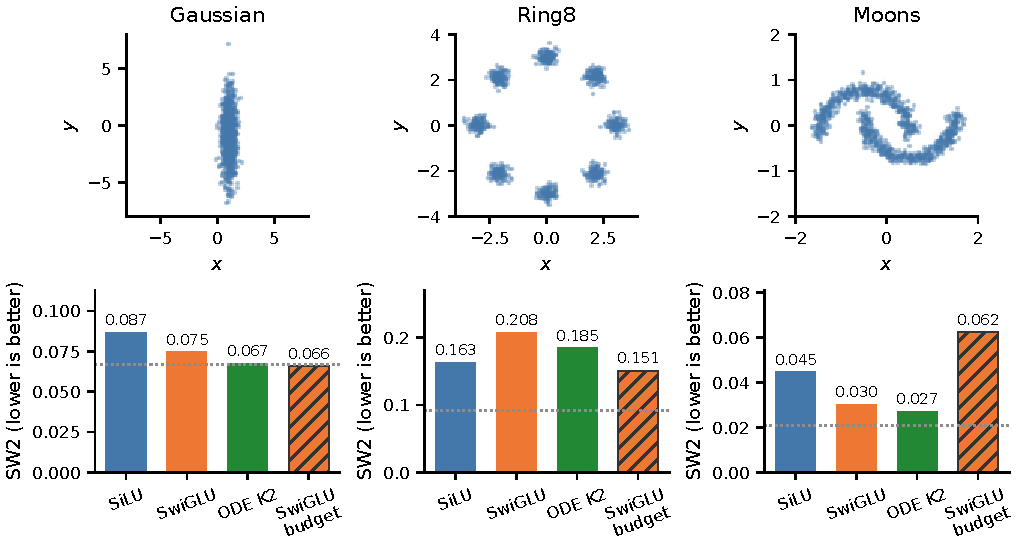
\includegraphics[width=\linewidth]{figures/01-data-and-comparison.pdf}
\caption{\textbf{Targets and the budget comparison.} Top: the first 1,000 held-out target points from each actual dataset. Bottom: fixed-endpoint $\sw$ with seed 0. All solid bars use 5,000 updates; the hatched SwiGLU bar uses 6,572 to match the ODE $K=2$ forward-linear-MAC budget. Dotted lines show target-versus-target subset distances as finite-sample references, not attainable lower bounds. Compare architectures within a dataset; vertical scales differ across datasets.}
\label{fig:overview}
\end{figure}
\begin{figure}[!ht]
\centering
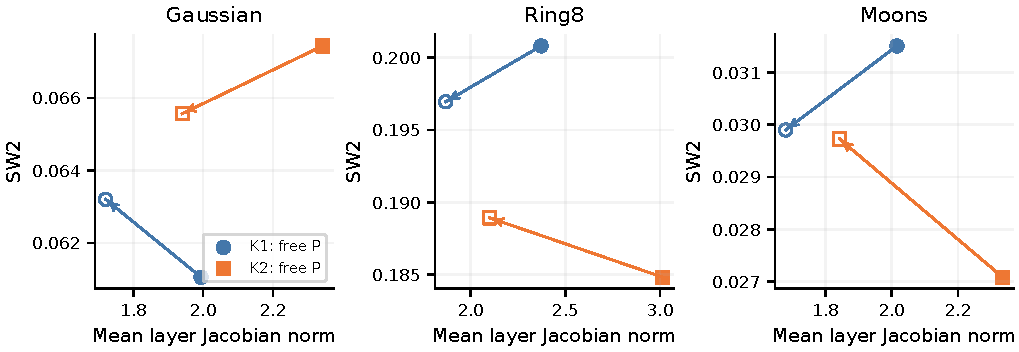
\includegraphics[width=\linewidth]{figures/02-spectral-cap.pdf}
\caption{\textbf{Spectral cap: smaller internal sensitivity is not uniformly better generation.} Each arrow links a free-$P$ model (filled marker) to a separately trained capped model (open marker) at the same order. Horizontal values average local spectral norms of the full ODELayer Jacobian over 16 probes and six layers; vertical values are $\sw$ at 5,000 updates. The cap always moves left but does not always move down. Seed 0; no across-seed error bars.}
\label{fig:cap}
\end{figure}

\clearpage
\section*{Visualizations: gating and Taylor order}
\begin{figure}[!ht]
\centering
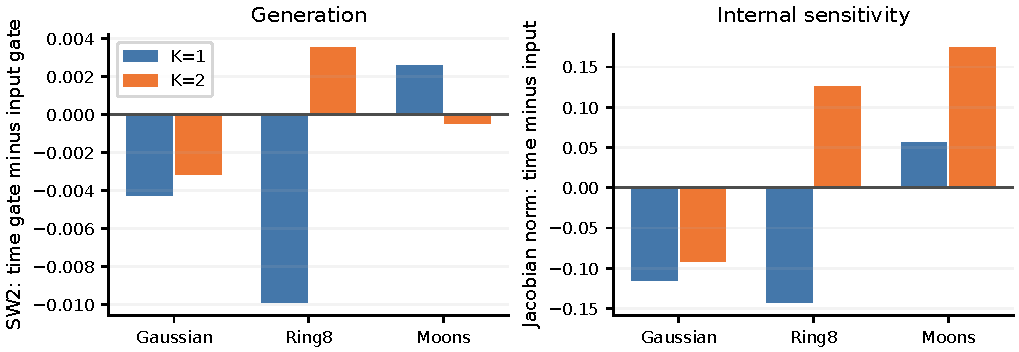
\includegraphics[width=\linewidth]{figures/03-gate-intervention.pdf}
\caption{\textbf{Time gating is not a uniform improvement.} Differences are time-gated minus input-gated results after separate 5,000-update training runs. Negative values mean lower $\sw$ (left) or lower full-layer Jacobian norm (right). The gate-derivative contribution is exactly zero for time gating, yet the full-layer norm can increase as the learned operators adapt. All runs use seed 0.}
\label{fig:gate}
\end{figure}
\begin{figure}[!ht]
\centering
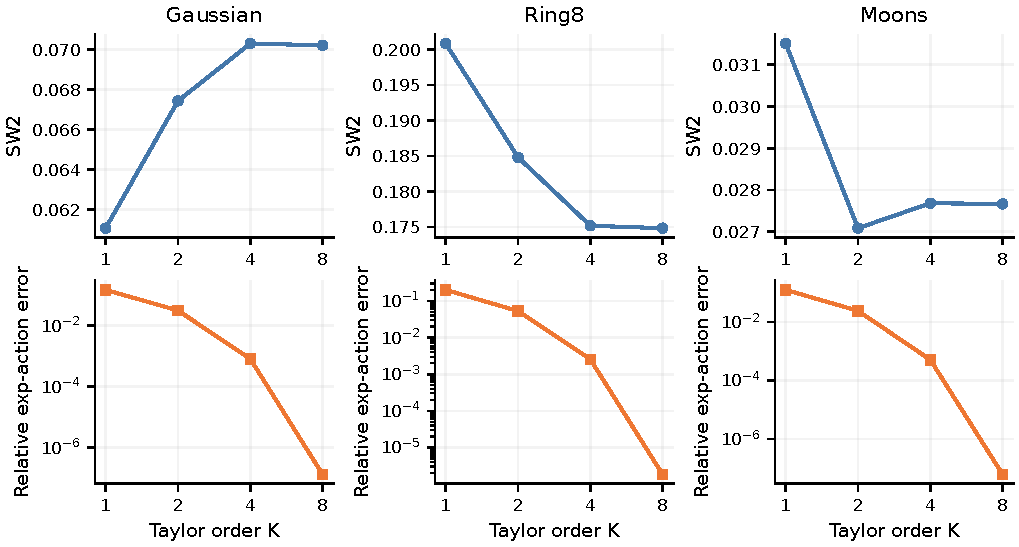
\includegraphics[width=\linewidth]{figures/04-order.pdf}
\caption{\textbf{Exponential accuracy improves much more than generation from $K=4$ to $K=8$.} Top: $\sw$ for separately trained input-gated models at the fixed 5,000-update endpoint. Bottom: relative action discrepancy from the matrix exponential, averaged over 16 actual hidden probes per layer and six layers. The exponential reference uses each model's own learned $P$ and gate. This is not a fixed-$P$ order intervention. Seed 0; logarithmic error axis.}
\label{fig:order}
\end{figure}

\clearpage
\section*{Visualizations: learned operators and a Ring8 case study}
\begin{figure}[!ht]
\centering
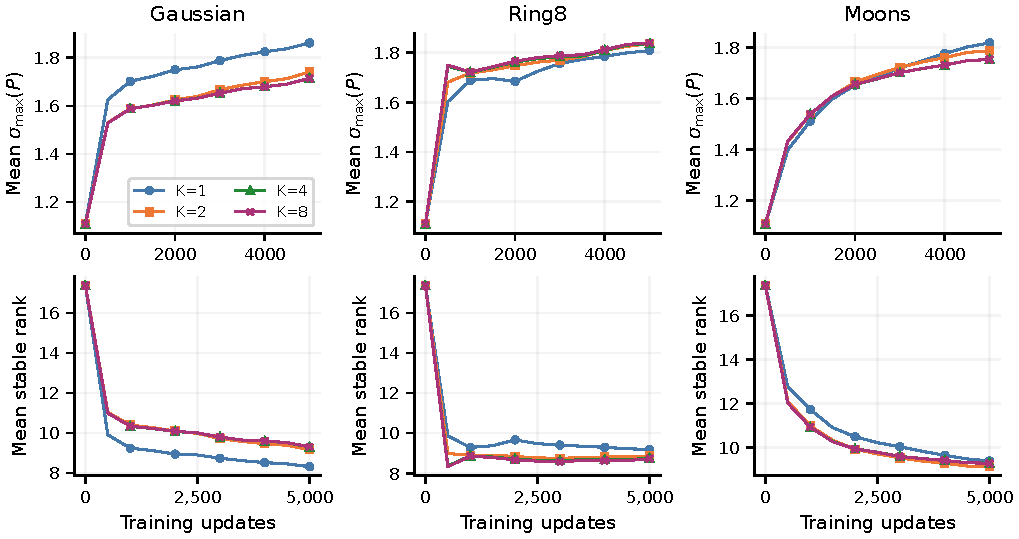
\includegraphics[width=\linewidth]{figures/05-p-trajectories.pdf}
\caption{\textbf{Training strengthens the leading directions of $P$.} Top: largest singular value. Bottom: stable rank. Each curve is a six-layer mean from one input-gated training trajectory; these means do not estimate uncertainty. All orders begin from identical weights. $K=4$ and $K=8$ are nearly superimposed. Seed 0; stable rank is a concentration measure, not the number of nonzero singular values.}
\label{fig:trajectory}
\end{figure}
\begin{figure}[!ht]
\centering
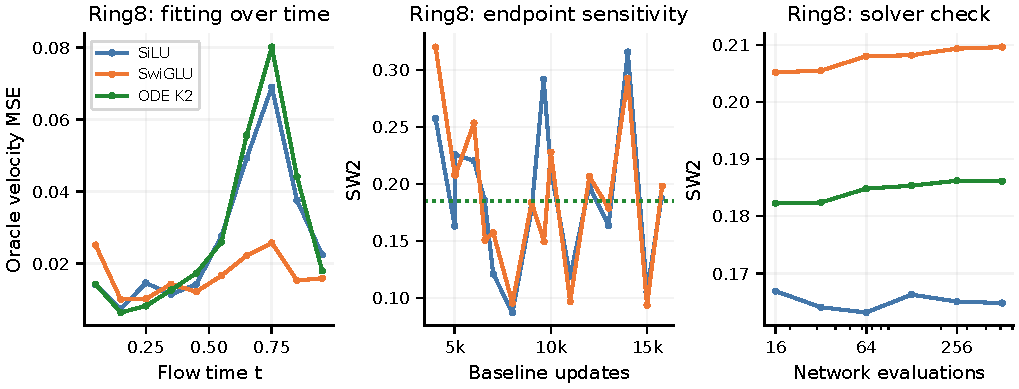
\includegraphics[width=\linewidth]{figures/06-ring8-case.pdf}
\caption{\textbf{Ring8 illustrates three limits of endpoint comparisons.} Left: binned oracle velocity MSE on held-out interpolated points shows different error timing for SiLU, SwiGLU, and ODE $K=2$. Middle: actual long-run baseline checkpoints fluctuate; the dotted green line is the ODE $K=2$ score at 5,000 updates, not an ODE training curve. Right: changing the external solver's evaluation count preserves the main ranking. Two evaluations equal one Heun step. All panels use seed 0; connected checkpoints are not independent repetitions.}
\label{fig:case}
\end{figure}
\end{document}
